\section{物理参数的无量纲化}
\frame{\frametitle{物理参数的无量纲化}
\begin{table}[!htb]
\centering
\caption{物理量的无量纲过程}
\begin{tabular}{|c|c|c|}
\hline 
量纲& 无量纲量 & 物理量\tabularnewline
\hline 
\hline 
Energy & $E^{*}=E/\varepsilon$ & $E=\varepsilon E^{*}$\tabularnewline
\hline
Length & $L^{*}=L/\lambda$ & $L=\lambda L^{*}$\tabularnewline
\hline
Mass & $m^{*}=m/\mu$ & $m=\mu m^{*}$\tabularnewline
\hline 
Temperature & $T^{*}=k_{B}T/\varepsilon$ & $T=\varepsilon T^{*}/k_{B}$\tabularnewline
\hline 
Density & $\rho^{*}=\lambda^{3}\rho$ & $\rho=\rho^{*}/\lambda^{3}$\tabularnewline
\hline 
Force & $F^{*}=\lambda F/\varepsilon$ & $F=\varepsilon F^{*}/\lambda$\tabularnewline
\hline 
Pressure & $P^{*}=\lambda^{3}P/\varepsilon$ & $P=\varepsilon P^{*}/\lambda^{3}$\tabularnewline
\hline 
Time & $t^{*}=t\sqrt{\varepsilon/\mu}/\lambda$ & $t=t^{*}\lambda\sqrt{\mu/\varepsilon}$\tabularnewline
\hline 
\end{tabular}
\end{table}
加速度的无量纲化$\displaystyle
g^{*}=\frac{F^{*}}{m^{*}}=\frac{\lambda F}{\varepsilon}\frac{\mu}{m}=\frac{\lambda\mu}{\varepsilon}g
$
}

\frame{\frametitle{实验构造}
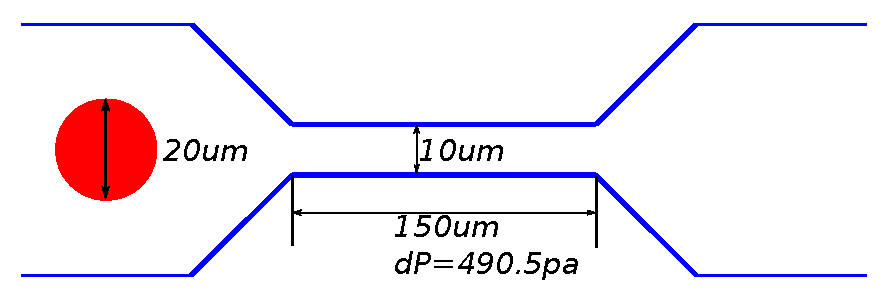
\includegraphics[width=\textwidth]{conf.pdf}
}

\frame{\frametitle{实验中的物理量数值}
\begin{table}[!htb]
\begin{tabular}{|c|c|}
\hline 
 参数& 物理值\tabularnewline
\hline 
\hline 
diameters of the cell & $20\pm5\mu m$\tabularnewline
\hline 
\hline 
diameters of the nucleus & $15\pm5\mu m$\tabularnewline
\hline 
\hline 
temperature & 22-24$^{\circ}C$\tabularnewline
\hline 
\hline 
cortical stiffness & 0.01dyn/cm(0.005-0.035dyn/cm)\tabularnewline
\hline 
\hline 
Elasticity & 0.001dyn/cm\textasciicircum{}2\tabularnewline
\hline 
\hline 
pressure & $\Delta p$=490.5pa, 3.33pa/um\tabularnewline
\hline 
\end{tabular}
\end{table}

加速度与压差的关系
\[
g = \frac{3.33 \mathrm{pa}/\mu \mathrm{m} \times S \Delta h}{S \Delta h \rho} 
= \frac{3.33\times 10^6 \mathrm{pa}/\mathrm{m}}{1\times 10^3 \mathrm{kg/m^3}}
= 3.33X10^3m/s^2
\]
}


\frame{\frametitle{物理参数的无量纲化}
选取体系的单位能量, 长度, 质量分别为
\[
\varepsilon=k_{B}T=1.381\times 10^{-23}\times(23+273.15)=4.0898\times 10^{-21}\mathrm{J}
\]
\[
\lambda=1\mu \mathrm{m}
\]
\[
\mu=1\times10^{3}kg/m^{3}\times(1\times10^{-6} \mathrm{m})^{3}/4=2.5\times10^{-16}kg
\]

加速度的无量纲化
\[
g^{*}=\frac{\lambda\mu}{\varepsilon}g = \frac{1\times10^{-6}\mathrm{m}\times 2.5\times 10^{-16}\mathrm{kg}}{4.0898\times 10^{-21}\mathrm{J}} \times 3.33X10^3\mathrm{m/s^2}= 203.56
\]
}
